\documentclass[11pt, a4paper]{article}

% --- UNIVERSAL PREAMBLE BLOCK ---
\usepackage[a4paper, top=2.5cm, bottom=2.5cm, left=2cm, right=2cm]{geometry}
% \usepackage{fontspec} % Removed: Requires XeLaTeX or LuaLaTeX
% \usepackage[english, bidi=basic, provide=*]{babel} % Removed: Part of fontspec setup
% \babelprovide[import, onchar=ids fonts]{english} % Removed
% \babelfont{rm}{Noto Sans} % Removed

% --- Fallback for pdfLaTeX environments ---
\usepackage[utf8]{inputenc} % Handle UTF-8 source code
\usepackage[T1]{fontenc}    % Use modern font encoding
\usepackage[english]{babel} % Standard babel package for pdflatex
% --- END PREAMBLE BLOCK ---

\usepackage{amsmath} % For math symbols
\usepackage{pgfplots} % For creating plots
\usepackage{booktabs} % For nice tables
\pgfplotsset{compat=1.18} % Use a modern version of pgfplots

\begin{document}

\section*{Insulation Wear: PVC vs. XLPE}

This chart shows the exponential decay in relative insulation resistance as operating temperature increases. The decay coefficients are adjusted to show a more pronounced curve, especially beyond the maximum operating temperatures. Note how XLPE's resistance decays slower and it remains functional at a higher maximum temperature.

\begin{figure}[h!]
\centering
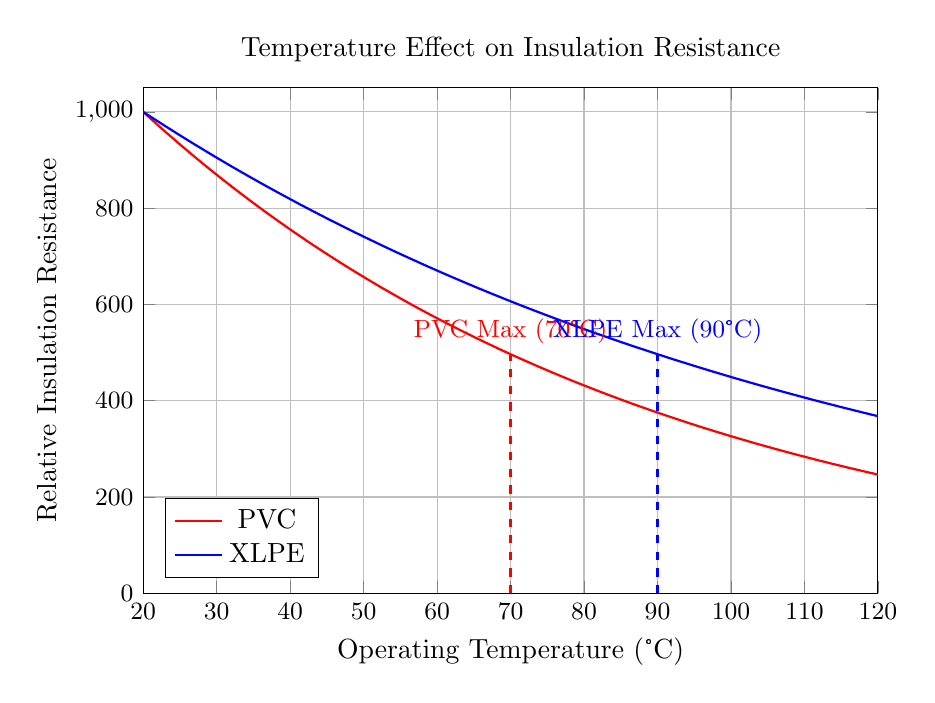
\begin{tikzpicture}
\begin{axis}[
    width=0.9\textwidth,
    height=8cm,
    title={Temperature Effect on Insulation Resistance},
    xlabel={Operating Temperature (°C)},
    ylabel={Relative Insulation Resistance},
    xmin=20, xmax=120,
    ymin=0, ymax=1050, % Adjusted ymax slightly
    legend pos=south west, % Moved legend to avoid overlap
    grid=major,
    ticklabel style={font=\small},
]

% Plot PVC - Adjusted alpha for moderate decay before 70C
\addplot[
    domain=20:120,
    samples=100,
    color=red,
    thick,
] {1000 * exp(-0.014 * (x - 20))}; % Used alpha = 0.014
\addlegendentry{PVC}

% Plot XLPE - Adjusted alpha for moderate decay before 90C
\addplot[
    domain=20:120,
    samples=100,
    color=blue,
    thick,
] {1000 * exp(-0.010 * (x - 20))}; % Used alpha = 0.010
\addlegendentry{XLPE}

% Max Temp Lines - Drawn up to the approximate resistance value at max temp
\draw[red, dashed, thick] (axis cs:70, 0) -- (axis cs:70, {1000 * exp(-0.014 * (70 - 20))}) % Ends near the curve at T=70
    node[above, pos=1, anchor=south, font=\small] {PVC Max (70°C)};

\draw[blue, dashed, thick] (axis cs:90, 0) -- (axis cs:90, {1000 * exp(-0.010 * (90 - 20))}) % Ends near the curve at T=90
    node[above, pos=1, anchor=south, font=\small] {XLPE Max (90°C)};

\end{axis}
\end{tikzpicture}
\caption{Comparison of insulation resistance decay for PVC and XLPE (More Curved Decay Model).}
\end{figure}

\clearpage

\section*{Economic Comparison of Conductors}

These charts illustrate the trade-off between initial cost and estimated 30-year operating cost for different conductor materials.

\begin{figure}[h!]
\centering
% Bar Chart 1: Initial Cost
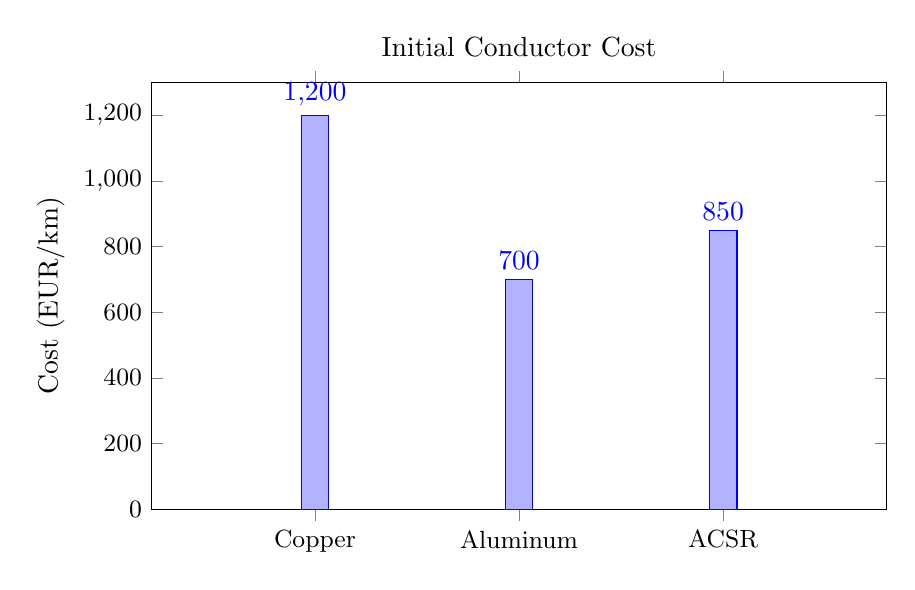
\begin{tikzpicture}
\begin{axis}[
    ybar,
    width=0.9\textwidth,
    height=7cm,
    title={Initial Conductor Cost},
    ylabel={Cost (EUR/km)}, % Changed € symbol to EUR
    symbolic x coords={Copper, Aluminum, ACSR},
    xtick=data,
    nodes near coords,
    nodes near coords align={vertical},
    ymin=0,
    ymax=1300, % Adjusted ymax for better spacing
    enlarge x limits=0.4,
    ticklabel style={font=\small} % Removed trailing comma here
]
\addplot coordinates {
    (Copper, 1200)
    (Aluminum, 700)
    (ACSR, 850)
};
\end{axis}
\end{tikzpicture}
\caption{Initial material cost per kilometer.}
\end{figure}

\begin{figure}[h!]
\centering
% Bar Chart 2: Estimated 30-Year Operating Cost
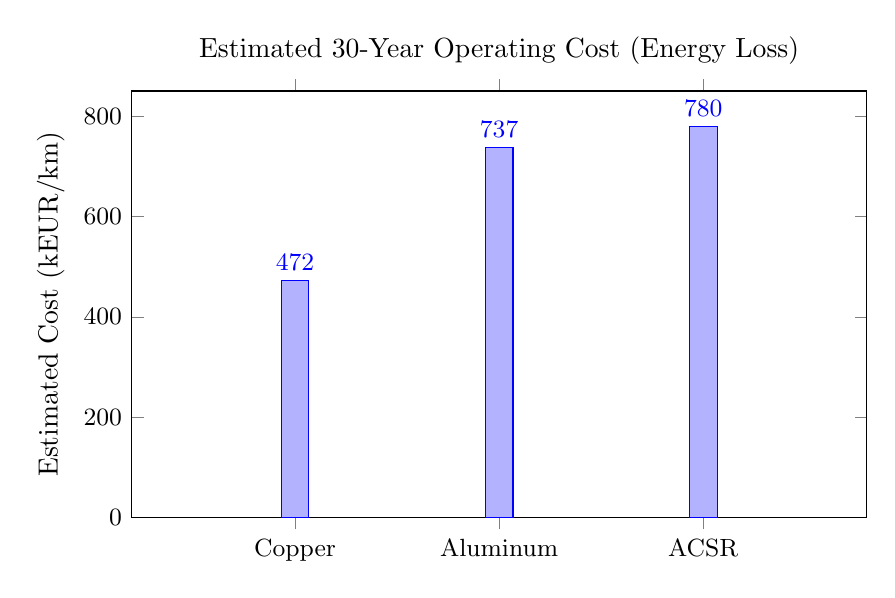
\begin{tikzpicture}
\begin{axis}[
    ybar,
    width=0.9\textwidth,
    height=7cm,
    title={Estimated 30-Year Operating Cost (Energy Loss)},
    ylabel={Estimated Cost (kEUR/km)}, % Changed label
    symbolic x coords={Copper, Aluminum, ACSR},
    xtick=data,
    nodes near coords,
    nodes near coords style={ % Adjusted formatting
        /pgf/number format/fixed,
        /pgf/number format/precision=0,
        font=\small
    },
    nodes near coords align={vertical},
    ymin=0,
    ymax=850, % Adjusted ymax based on new values
    enlarge x limits=0.4,
    ticklabel style={font=\small}, % Kept comma here as it's correct
]
% Estimated Costs in kEUR (Calculations based on assumptions in description)
\addplot coordinates {
    (Copper, 472)      % Roughly 472,020 EUR
    (Aluminum, 737)    % Roughly 736,532 EUR
    (ACSR, 780)        % Roughly 779,595 EUR
};
\end{axis}
\end{tikzpicture}
\caption{Estimated 30-year operating cost due to energy losses, based on assumed load (100A), area (50mm²), temp (50°C), and price (€0.15/kWh). For comparative purposes only.\protect\footnote{Energy loss calculation: Power loss per phase is $P_{loss} = I^2 R$. For a balanced 3-phase system, total power loss is $P_{total} = 3 \times I^2 R$. Total energy loss over a period is $E_{loss} = P_{total} \times \text{time} = 3 \times I^2 R \times \text{time}$. $R$ is the resistance per km at the assumed operating temperature.}}
\end{figure}

\end{document}

